%
% Szakdolgozatminta az Eszterházy Károly Katolikus Egyetem
% matematika illetve informatika szakos hallgatóinak.
%

\documentclass[
% opciók nélkül: egyoldalas nyomtatás, elektronikus verzió
% twoside,     % kétoldalas nyomtatás
% tocnopagenum,% oldalszámozás a tartalomjegyzék után kezdődik
]{thesis-ekf}
\usepackage[T1]{fontenc}
\PassOptionsToPackage{defaults=hu-min}{magyar.ldf}
\usepackage[magyar]{babel}
\usepackage{mathtools,amssymb,amsthm,pdfpages}
\footnotestyle{rule=fourth}

\newtheorem{tetel}{Tétel}[chapter]
\theoremstyle{definition}
\newtheorem{definicio}[tetel]{Definíció}
\theoremstyle{remark}
\newtheorem{megjegyzes}[tetel]{Megjegyzés}

\begin{document}

\institute{Matematikai és Informatikai Intézet}
\title{Mesterséges intelligencia számítógépes játékokban}
\author{Herbák Marcell\\Programtervező Informatikus BSc}
\supervisor{Dr. Kovásznai Gergely\\Egyetemi docens}
\city{Eger}
\date{2025}
\maketitle

\tableofcontents

\chapter{Bevezetés}

\section{Játék ismertetése}

\begin{figure}[h!]
	\centering
	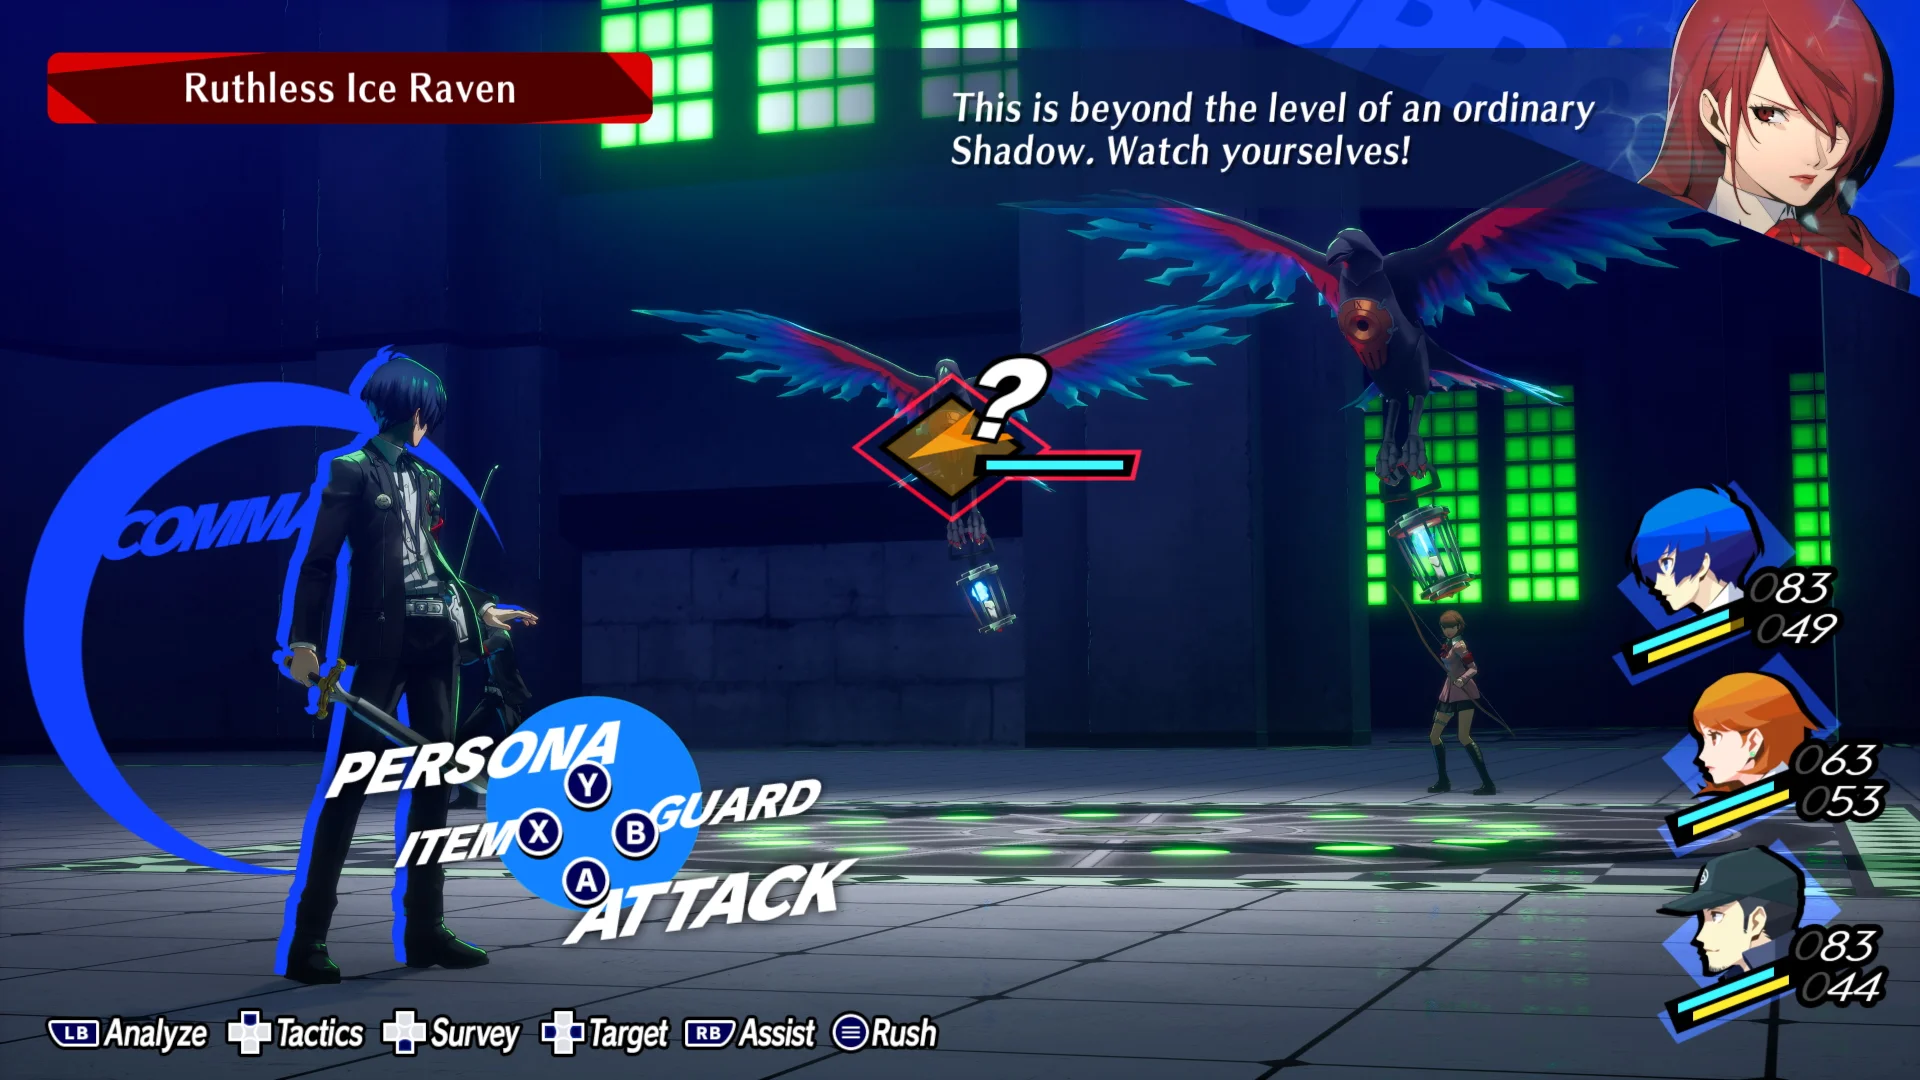
\includegraphics[width=14cm]{./pictures/persona3_xbox.png}
	\caption{Persona 3 Reload}
	\label{persona3}
\end{figure}

\subsection{Játék ötlete}

Szakdolgozatom programjaként egy olyan játékot szerettem volna készíteni, amely nem csak jól implementálható, hanem amivel szabadidőmet is szívesen töltöm. Választásom végül is egy körökre osztott stratégiai játék elkészítésére esett. Ötletadónak, az általam kedvelt videójáték szériát, a Persona játékokat választottam. Az első Persona játék közel 30 éve jelent meg a Shin Megami Tensei szériának spin--off-jaként, így a játékok működésben és történetben bár eltérőek a modern megjelenésektől, jelenleg legfrissebb 2024-ben kiadott (\ref{persona3} ábra) Persona 3 Reload-tól, a játék fő mechanikája nem változott: a játékos karakterei csatába kerülnek egy fix számú, hasonló képességű ellenfelekkel szembe. Ezekben a játékokban, különleges képességekkel rendelkező, úgynevezett Personákkal harcolnak a különböző szereplők.\cite{Persona,Persona3}

Bár a modern játékokban nem alkalmazzák már, a Revelations: Persona harcrendszere (\ref{persona1} ábra) rendelkezett mezőkre felbontott csatatérrel, amelyeknél még a támadásoknak volt egy bizonyos maximális távolsága. Ezek alapján szerettem volna egy olyan játékteret készíteni, ahol a játékosnak nem csak a támadásának a távolságát kell figyelembe vennie, hanem a helyét is a csatatéren. \cite{Persona1,Persona1Gameplay}
\begin{figure}[h!]
	\centering
	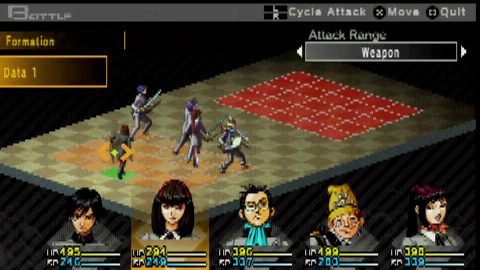
\includegraphics[width=13cm]{./pictures/persona_psp.png}
	\caption{Revelations: Persona}
	\label{persona1}
\end{figure}

\subsection{Játék szabályok} \label{rules}

A játék egy fixált méretű, négyzetekből álló, 7x10 nagyságú táblán folyik. A játékot kettő játékos tudja játszani, melyből a szakdolgozatomban az egyik játékos a mesterséges intelligencia lesz. Mindegyik játékos rendelkezik karakterekkel, amelynek kezdő mennyisége a játék indítása előtt kiválasztható. Mindkét játékos rendelkezik minimum 1, maximum pedig 3 karakterrel. A karakterek mennyisége játékosonként eltérő lehet, nem szükséges mindkét játékosnak ugyanazzal a karakter mennyiséggel kezdenie. Az egyik játékos karakterei (több karakter esetén függőlegesen egy mező kihagyással) a 2. oszlopban, a másik játékos karakterei pedig a 9. oszlopban kezdenek. A táblán léteznek akadályozó mezők, amelyekre a játékosok nem léphetnek, illetve nem támadhatják meg. 

A játék során a játékosok egymás után jönnek, egy körben az összes karakterükkel végre kell hajtaniuk egy interakciót. Ez a két interakció \emph{lépés} és \emph{támadás} lehet. Lépés során a karakterükkel egy mezőt léphetnek a négy irány közül valamelyik irányba: fel, le, balra vagy jobbra. A játékos karaktere nem léphet olyan mezőre, amelyen már áll egy másik saját karakter, egy ellenfél karakter vagy egy akadály. Támadás során a játékos egy mezőn belül támadhat négy irány közül valamelyik irányba. A játékos karaktere nem támadhatja meg a saját karakterét, illetve nem támadhat üres vagy akadály mezőt. A karakterek rendelkeznek életerővel, minden karakter a játék kezdésekor 10 életerőponttal kezd. Támadás során a megtámadott karakter elveszít 1 életerő pontot. Amennyiben a játékos minden karakterére végrehajtott egy interakciót, a játékos átadja a körét a másik játékosnak. A játékosoknak minden körben kötelező valamelyik interakciót végrehajtaniuk mindegyik karakterrel végrehajtani, illetve ha egy karakter interakcióját jóvá hagyták, azt vissza már nem vonhatják.

Egy karakter, amennyiben elveszíti összes életerejét, eltűnik a tábláról, mezője felszabadul, illetve innentől kezdve azzal nem tud a játékos interakciót végrehajtani és nem hozhatja vissza.
 
A játékos célja, hogy ellenfele összes karakterét eltüntesse a tábláról. A játékot az a játékos nyeri, akinek marad legalább 1 karaktere a táblán, legalább 1 életerővel.

\chapter{Mesterséges intelligencia}

\section{Története}

A mesterséges intelligencia története az 1930-as években vett rohamos lépéstempót Alan Turing és John McCarthy munkásságával.

\begin{figure}[h!]
	\centering
	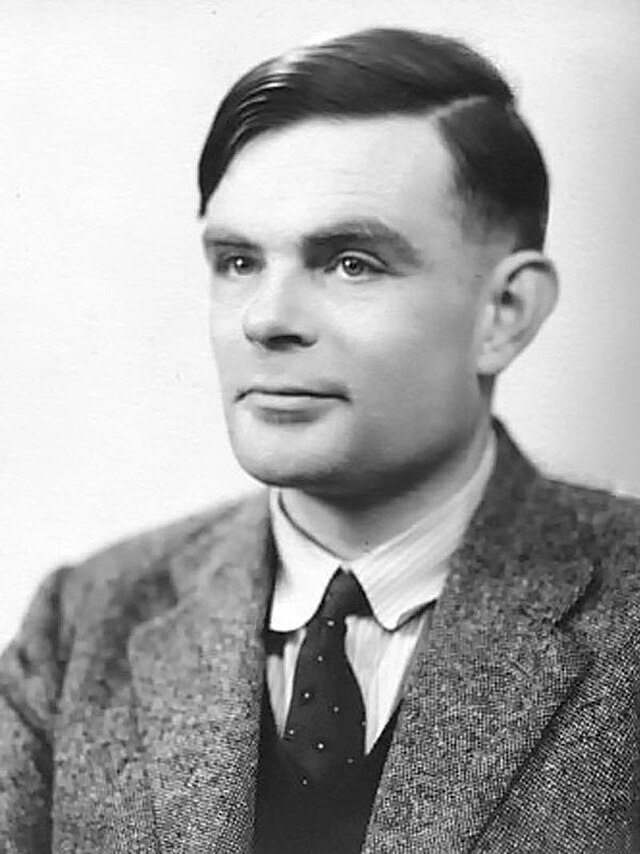
\includegraphics[width=7cm]{./pictures/Alan_Turing.jpg}
	\caption{Alan Turing}
	\label{Turing}
\end{figure} 

\textsc{Alan Turing} (1912--1954) az 1930-as évek elején megalkotta a Turing-gépet \textsc{Kurt Gödel} (1906--1978) munkássága alapján, amely a modern számítógépek elméleti alapját képezte. 1950-ben publikálta a ''Computing Machinery and Intelligence'' című tanulmányát, amelyben felvetette a gépek gondolkodási képességének kérdését, és bevezette a híres Turing-tesztet, amely azt vizsgálja, hogy egy gép képes-e emberihez hasonló intelligens viselkedésre. \cite{AlanTuring,CMI}

\textsc{John McCarthy} (1927–-2011) amerikai számítástechnikai és kognitív tudós volt, akit a mesterséges intelligencia egyik alapítójaként tartanak számon. Ő alkotta meg a "mesterséges intelligencia" (artificial intelligence) kifejezést az 1956-os Dartmouth Konferencián, amelyet ő szervezett, és amelyet az MI hivatalos születésnapjaként tartanak számon. McCarthy 1958-ban kifejlesztette a Lisp programozási nyelvet, amely a mesterséges intelligencia-kutatás egyik legfontosabb eszközévé vált. Emellett jelentős hatással volt az ALGOL nyelv tervezésére, népszerűsítette az időosztásos rendszereket, és feltalálta a szemétgyűjtést (garbage collection). 

\begin{figure}[h!]
	\centering
	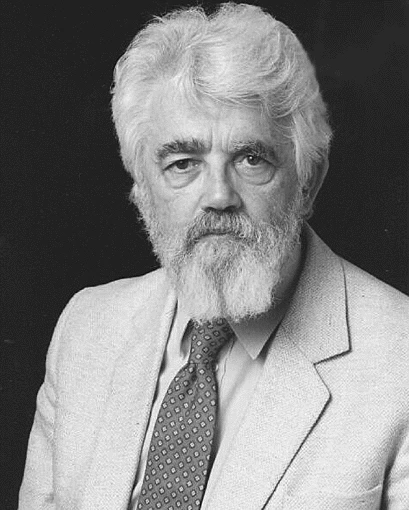
\includegraphics[width=5cm]{./pictures/John_McCarthy.png}
	\caption{John McCarthy}
	\label{McCarthy}
\end{figure}

McCarthy munkássága jelentős hatással volt a mesterséges intelligencia fejlődésére. Az 1960-as és 1970-es években az MI-kutatás optimizmusa után nehéz időszak jött, amikor a fejlődés lelassult a korlátozott számítási kapacitás és a finanszírozási problémák miatt. Azonban McCarthy és kortársai kitartása hozzájárult ahhoz, hogy az MI napjainkban az egyik legdinamikusabban fejlődő területté váljon. Az utóbbi évtizedekben a gépi tanulás, a neurális hálózatok és a mélytanulás forradalmasították az MI-t, amely ma már számos területen, például az orvostudományban, az iparban és az önvezető autókban is kulcsszerepet játszik. \cite{JohnMcCarthy}

\section{Játékelmélet}

A játékelmélet a matematika egyik, tudományágak közé egyértelműen nehezen besorolható (interdiszciplináris) ága, mely olyan kérdésekkel foglalkozik, hogy mi az ésszerű (racionális) viselkedés olyan helyzetekben, ahol minden résztvevő döntéseinek eredményét befolyásolja a többi résztvevő lehetséges választásai, röviden a stratégiai problémák elmélete. A játékelmélet alapjait Neumann János fektette le ''Zur Theorie der Gesellschaftsspiele'' című 1928-as munkájában \cite{Neumann}, majd Oskar Morgenstern neoklasszikus matematikus-közgazdásszal közösen megírta a „Játékelmélet és gazdasági viselkedés” című (The Theory of Games and Economic Behavior, 1944) művüket. \cite{Jatekelmelet,JatekelmeletEn} Ezen művek alapján a következő fogalmakat tisztáznunk kell \cite{NeumannOskar}:

\begin{itemize}
	\item A \emph{játék} a játékosok viselkedését és lényeges körülményeket meghatározó szabálysor által leírt folyamat.
	\item Az információs halmaz (ismeret) meghatározó szerepű. Ez azt jelenti, hogy az információs halmaz alapján különböző típusokat sorolhatunk fel, például a \emph{tökéletes információs} és \emph{véges}, ahol minden résztvevő birtokolja az összes vonatkozó adatot (szabályok, lehetséges és korábbi események).
	\item Egy játék lehet két- vagy többszemélyes.
	\item Mikor a játékban a játékosok versengenek egymással, akkor \emph{nem kooperatív} játékról beszélünk.
	\item Zérusösszegű az a játék, amelyben a játékosok csak az ellenfelük nyereségük csökkentésével növelhetik nyereségüket.
	\item A játékost győzelemre, de minimum döntetlenre segítő módszere a \emph{stratégia}. Ilyenkor kihasználhatja az ellenfél érzékelt hibáit.
\end{itemize} 

\subsection{Minimax algoritmus}

A minimax elv olyan alkalmazott döntési szabály a játékelméletben, ami szerint azt a lehetőséget kell választani, ami minimalizálja a maximális veszteséget. Ezt az elvet felhasználhatjuk a kétfős zérusösszegű játékoknál, ami magába foglalja a két játékos szimultán döntéseit és a felváltva tett lépéseit is. \cite{MiniMaxEnWiki}

Formális definíció szerint a következőképpen tudjuk felírni a számítást:

\begin{equation*}
\overline{v_{i}}=\underset{{a_{-i}}}{\min} \underset{{a_{i}}}{\max} v_{i}(a_{i}, a_{-i})
\end{equation*}

A minimax érték azt fejezi ki, hogy egy játékos legrosszabb esetben mekkora értéket érhet el, ha a többi játékos a számára legkedvezőtlenebb stratégiát követi. Másképpen megfogalmazva, ez az a legnagyobb érték, amelyet a játékos garantáltan megszerezhet, ha ismeri a többi játékos lépéseit. 

Egy kétszemélyes játékban az egyik játékos a maximalizáló, aki a saját pontszámának maximalizálására törekszik, míg a másik a minimalizáló, aki a maximalizáló pontszámának minimalizálására törekszik. Az algoritmus úgy működik, hogy kiértékeli az összes lehetséges lépést mindkét játékos számára, előrejelzi az ellenfél válaszait, és kiválasztja az optimális lépést annak érdekében, hogy a lehető legjobb eredményt biztosítsa. \cite{MiniMaxGfG}

\subsection{Minimax alfa-béta vágással}

\chapter{Implementáció}

\section{Technológiák}

\subsection{Játékmotor}

A szakdolgozatom megvalósításához a Unity-t (korábban Unity3D) használom. A Unity egy világszerte ismert és használt videójáték-motor, amelyet a Unity Technologies fejleszt 2005 óta. A motor támogat több különböző platformot, például PC, videójáték konzolok és okostelefonok. Különösen kedvelik a kezdő játékfejlesztők a letisztult felülete és egyszerű használata miatt. Választásom azért esett a Unity-re, mert a szkriptekhez natívan támogatja a C\# nyelvet. A szakdolgozatomban a Unity-nek a 2022.3.32f1-es verzióját használom.

\begin{figure}[h!]
	\centering
	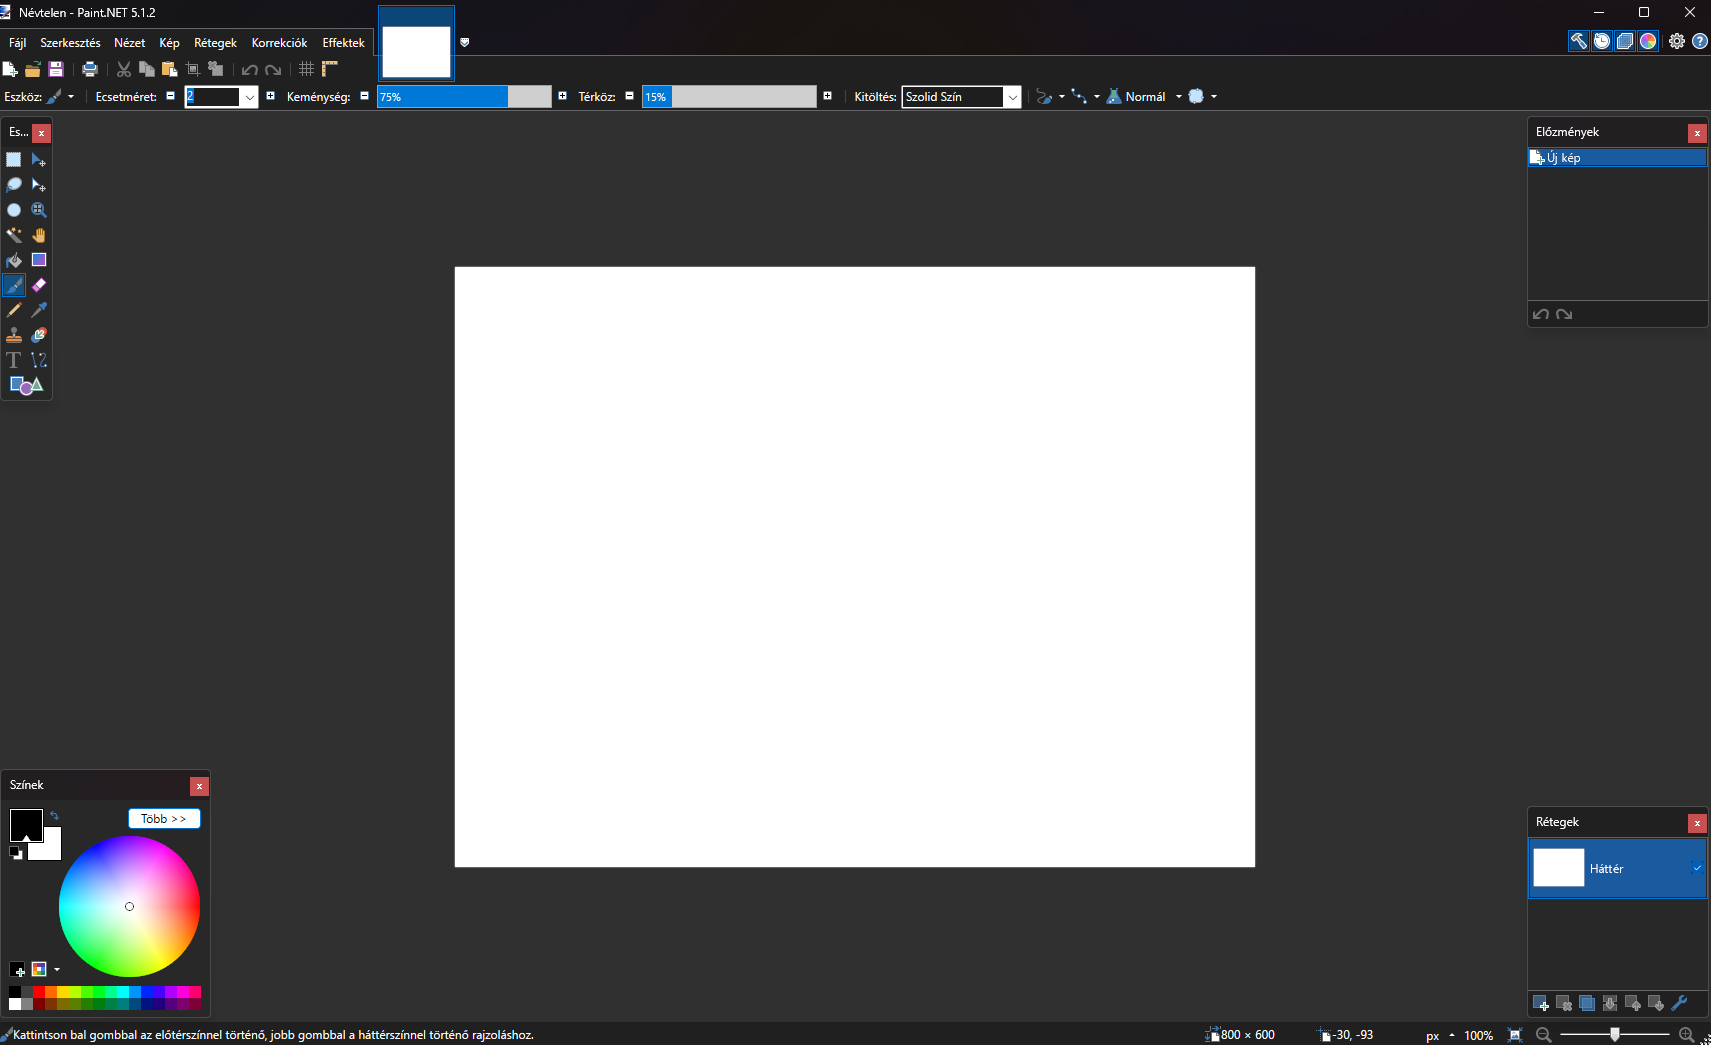
\includegraphics[width=15cm]{./pictures/paint_net.png}
	\caption{Paint.NET felülete}
	\label{PaintNET}
\end{figure}

\subsection{Grafikus szerkesztő}

A szakdolgozatomat a Unity-be beépített színeken és objektumokon kívül, általam készített pixelábrákat használok a karakterek képeként, amelyekhez a Paint.NET szoftvert használtam. A Paint.NET egy szabad licenszű, rasztergrafikus alkalmazás, amelyet a dotPDN fejleszt. A szakdolgozatom készítésekor 5.1.2 verzióját használtam a szoftvernek.

\section{Megjelenítés}

A játék készítésekor törekedtem a minimalista és könnyen vezérelhető kezelőfelületre. A Unity-ben úgynevezett \emph{scene}-ekre lehet osztani a játékot, legközelebbi példaként a \emph{WinForms} alkalmazásokban egy új \emph{form} létrehozásával lehet párhuzamba hozni ezt a megoldást. A WinForms, másik nevén Windows Forms egy Microsoft által kiadott, nyílt forráskódú szoftver, amely elsődleges céljának kliens alkalmazások fejlesztésére adtak ki Windows rendszerekre. \cite{winforms}

A játék három scene-ből épül fel: \emph{MenuScene}, \emph{GameScene} és \emph{EndScene}.

\subsection{MenuScene} \label{menusection}

\begin{figure}[h!]
	\centering
	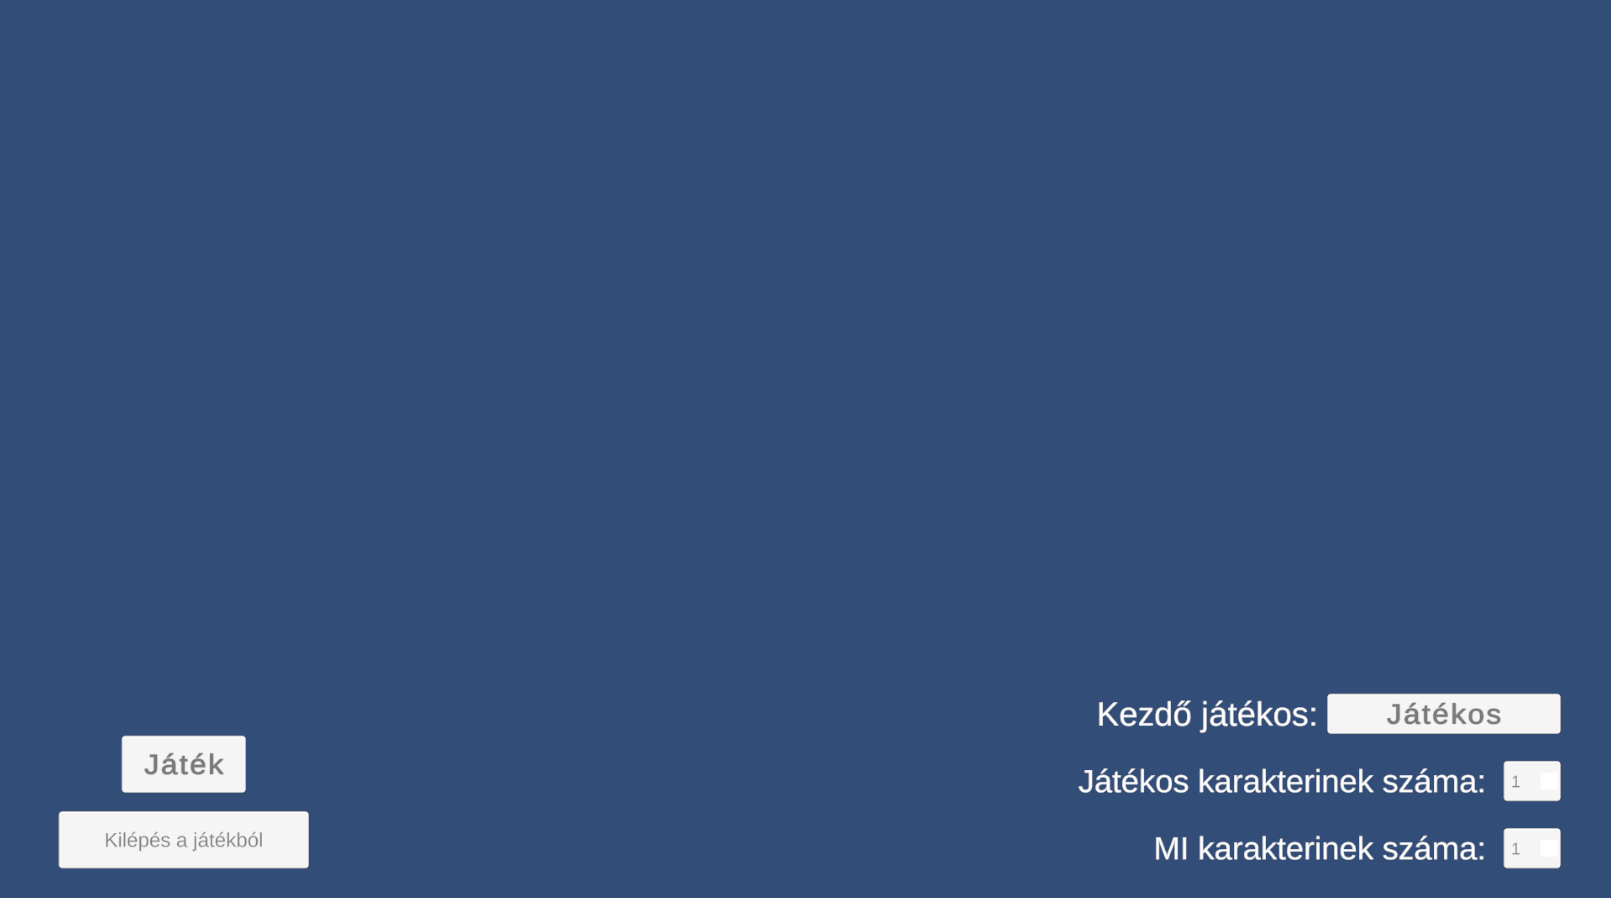
\includegraphics[width=15cm]{./pictures/game_menu.png}
	\caption{A játék menüjének felépítése}
	\label{menuscene}
\end{figure}

A \emph{MenuScene} az alap \emph{Camera} objektumon kívül tartalmaz egy \emph{Canvas} 2D-s objektumot. Ezen a felületen találhatóak a különböző funkciókat betöltő objektumok. A kép bal alsó sarkában található az \emph{ExitButton} nevű gomb objektum, amely névéhez illően kilép az alkalmazásból, felette található a \emph{PlayButton} gomb, amely a felhasználó által kiválasztott beállítások alapján elindítja a játékot. A képernyő jobb oldalán lehet találni a beállításokat módosító gombokat és karakterek számát kiválasztó \emph{Dropdown}\footnote{Legördülő lista} listákat. A gomb megnyomásával kiválaszthatja a játékos, hogy saját maga szeretné kezdeni a játékot vagy átadja a kezdés jogát a gépnek. A listákban a játékos ki tudja választani, hogy hány karakterrel induljon a játék, amely a korábban \aref{rules} szekcióban említett szabályok alapján ez akár négy karakterig is terjedhet. A \emph{MenuScene} felépítése \aref{menuscene} ábrán látható.

\subsection{GameScene}

A \emph{GameScene} az alkalmazás felületének leglényegibb része, ahol a játék folyik. A \emph{scene} tartalmaz kettő objektumot: \emph{GridObjectPrefab} nevű \emph{prefab}-et és egy canvas-t. 

A \emph{prefab} akár több \emph{GameObject}\footnote{A GameObject lényegében egy objektum, ami létezhet egy scene-n belül \cite{UnityDocsGameObject}} egyvelege, egy \emph{prefab}-ben a programozó tárolhat konfigurációt, mező értékeket illetve gyermek \emph{GameObject}-eket. Természetesen ezeket újra fel lehet használni, akár kódból példányosítani, illetve törölni is lehet őket a \emph{scene}-ből. \cite{UnityDocsPrefab} 

\begin{figure}[h!]
	\centering
	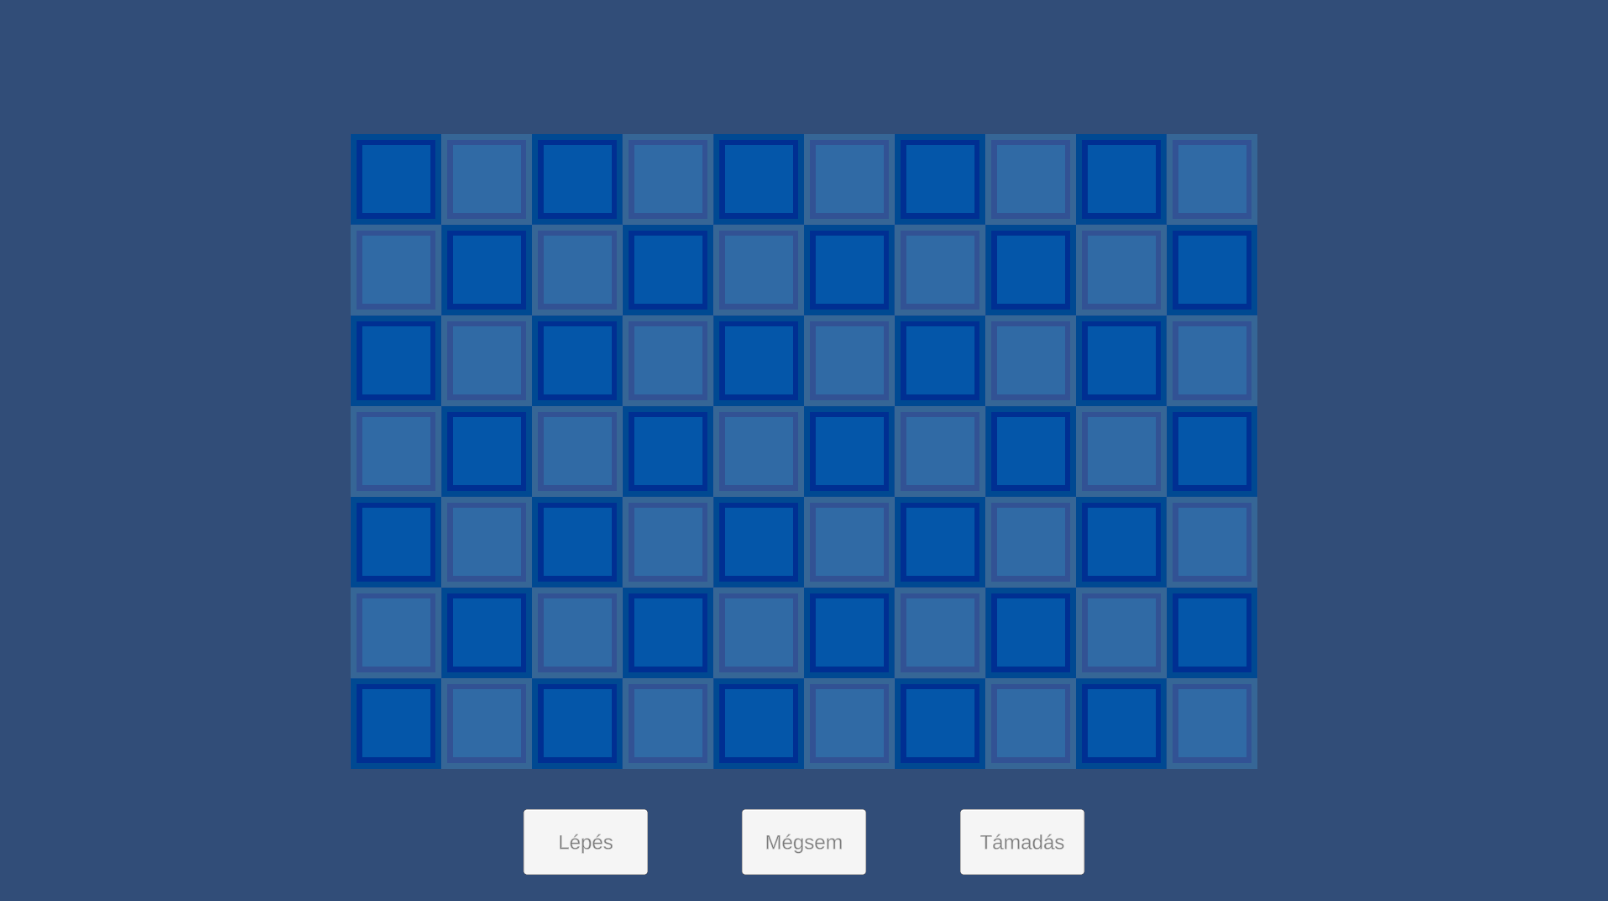
\includegraphics[width=15cm]{./pictures/game_grid.png}
	\caption{A játéktábla karakterek nélkül}
	\label{gamegrid}
\end{figure}

Ebben a \emph{prefab}-ben található a későbbi \ref{state} szekcióban tárgyalt állapottér megjelenítése, amelynek reprezentációs mátrixát egy \emph{Grid} objektummal implementálom. A \emph{Grid} objektum magában még nem a megjelenítést oldja meg, csupán a mátrix értékeit adom át a komponensnek átalakítva, ehhez még szükséges úgynevezett \emph{Tileset} objektumot létrehoznom. Ez a \emph{Tileset} objektum \emph{Tile} objektumokból áll, ami pedig kétféle négyzet alakú, 2D-s \emph{sprite} felületet vehet fel. Ez a felület függ az objektum koordinátájától, így sakktábla (\ref{gamegrid}~ábra) hatást keltve jelenik meg. 

A játék indulása során az állapottérből lekérdezett pozíciók alapján ezen prefab gyermekobjektumaként példányosítom a játékos és MI karakterek prefab-jeit. Ezek a prefab-ek tárolják magukban az állapottérben is tárolt adatokat (név, életerő, pozíció), illetve a karakter tulajdonosától függő sprite-ot.

A játék ideje alatt, ahogyan a karakterekkel lépnénk vagy támadnánk, a szabályoknak megfelelő módon a végrehajtható művelet céljának négyzete zöld színt kap, ha ez lehetséges, amennyiben nem, piros színt kap árnyalatnak (\ref{gamemove}~ábra). Amikor a játékos a felületen a kurzort mozgatja anélkül, hogy műveletet választana, akkor a négyzet, amelyen a kurzor található, szürke árnyalatot kap.

\begin{figure}[h!]
	\centering
	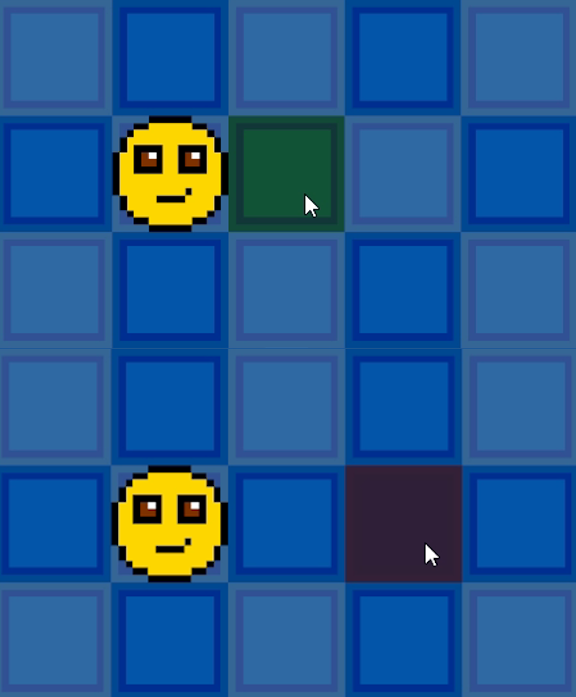
\includegraphics[width=6cm]{./pictures/game_move_tile.png}
	\caption{Példa helyes és helytelen lépésre}
	\label{gamemove}
\end{figure}

A scene másik összetevője egy canvas, amin találhatóak az életerőket tartalmazó vertikális csoportok és a vezérlő gombok. Három gomb közül kettő a játékteret befolyásoló erővel bír, a középső gomb arra szolgál, hogyha a játékos az akció végrehajtása előtt meggondolja magát, tudjon változtatni a műveleten, azonban amint kattintással jóváhagyta a játékos, ez a lehetőség megszűnik, tehát lépést nem lehet vissza vonni.

\begin{figure}[h!]
	\centering
	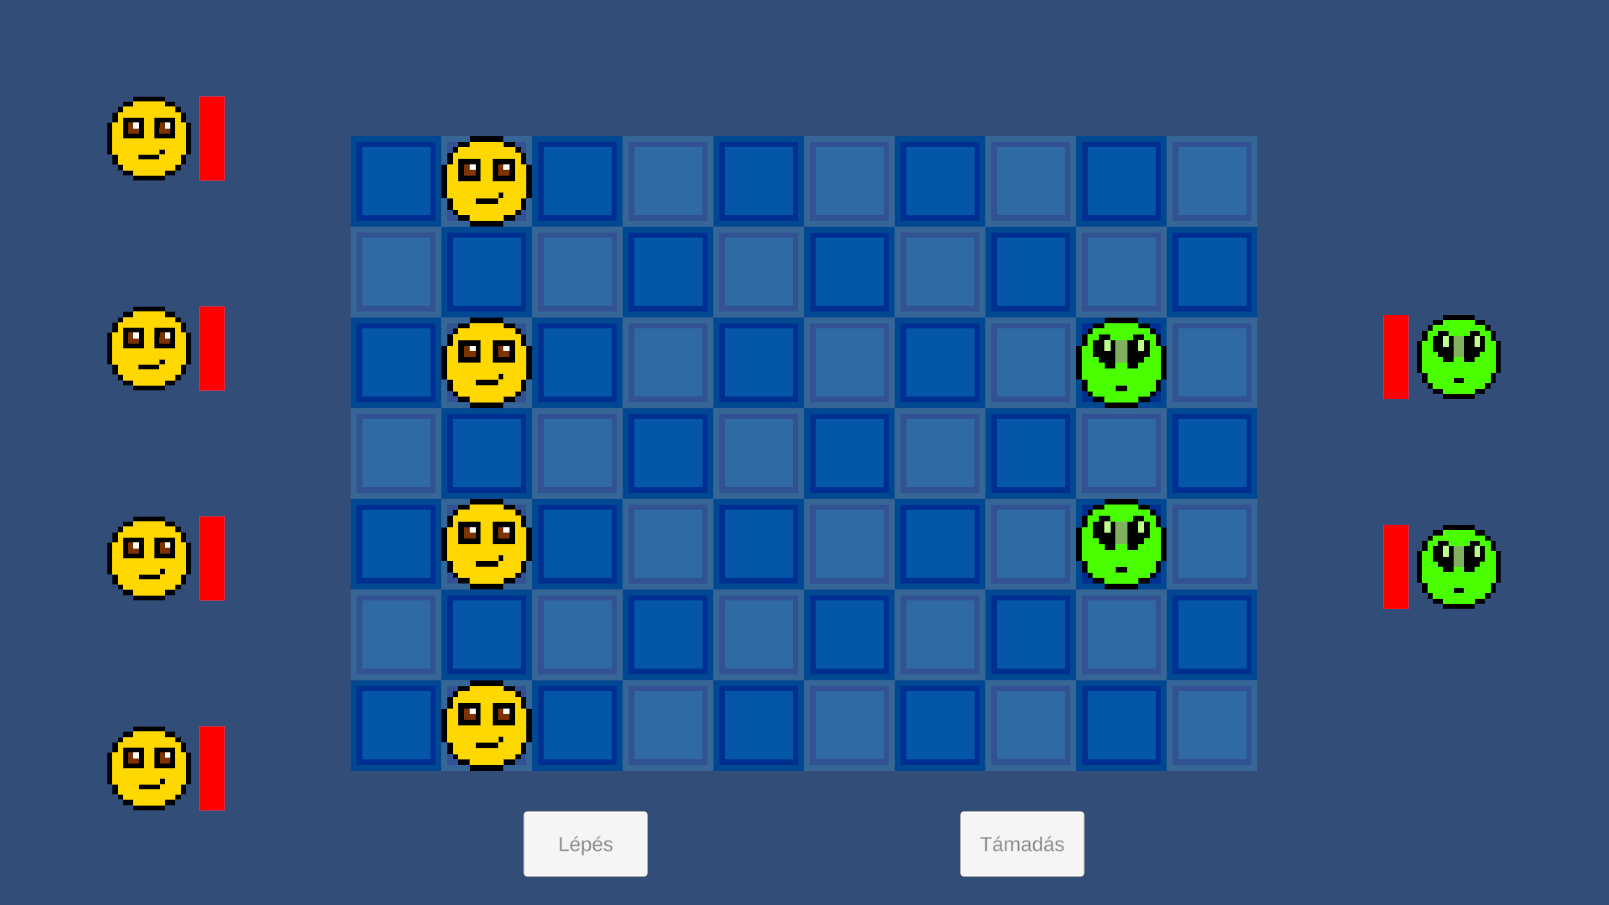
\includegraphics[width=14cm]{./pictures/game_health_ui.png}
	\caption{Játék egyik kezdőállapota}
	\label{game}
\end{figure}

A vertikális csoport tartalma a karakterek számától függően változik, tartalmazza a játékos vagy MI karaktereinek képét és két téglalap alakú 2D-s objektummal összerakott életerő csíkot, amely a karakterek életerejét mutatja. Ahogy a játék halad, amennyiben a játékos vagy MI karakterei életerőt vesztenek, a piros téglalap arányosan egyre kevesebb részt tölt ki az csíkból. Amennyiben a karakter elveszíti az összes életerejét, a prefab-je eltűnik a sávból.

\section{Állapottér} \label{state}

Az állapotterét kidolgozását a \emph{StateRepresentation} nevű osztályban oldottam meg. Ez az osztály tartalmaz egy \emph{FieldObject} típusú, hét sorból és tíz oszlopból álló mátrixot. A \emph{FieldObject} osztály az ősosztálya minden táblán szereplő entitásnak, ez alatt értendők az üres mezők, karakterek vagy akadályok. Az osztály példányai rendelkeznek egy azonosítóval és egy \emph{Vector2}\footnote{A Vector2 a Unity-n belüli megvalósítása a 2D-s vektoroknak és pontkoordinátáknak. \cite{UnityDocsVector2}} típusú pozícióval. Az osztály ezen kívül implementálja az \emph{ICloneable} interfészt, ezáltal mély klónozással \aref{minimax} szekcióban tárgyalt minimax algoritmus fel tudja használni. Ebből az osztályból származik a \emph{PlayerObject} osztály, amely már a játékos karakterek reprezentációját képezik a táblán. Ez az osztály az ősosztálybéli mezőkkel együtt tartalmazza még a karakterek életerejét, támadási erejét és egy logikai változót, amely a könnyű beazonosíthatóság érdekében eltárolja, hogy azt a karaktert az MI irányítja vagy sem.

Az állapottér osztálya ezen kívül tartalmaz még a működéshez szükséges metódusokat. A \emph{ChangeTurn()} eljárás az állapottér aktuális körét átállítja meghívás után a másik játékoséra. A \emph{GetStatus()} \emph{Status} felsorolás elemmel visszatérő függvény a játékosok karaktereinek száma alapján visszaad egy aktuális állapotot\footnote{Nem összekeverendő az állapottér reprezentáció és minimax algoritmus által visszaadott állapottal.}, amely szerint a játék jelenleg melyik fázisban tart. Lehetséges, hogy a \emph{játékos} vagy \emph{MI} nyert, valamint még folyamatban van a játék.

A működést befolyásoló metódusok közül az egyik legfontosabb a \emph{GetHeruistrics()} függvény, amely visszatér a paraméterben megadott játékos állapotának heurisztikai értékével. A függvény működéséről részletesebben \aref{heuristics} szekcióban olvashat. Ezeken kívül található több, a táblán különböző objektumok lekérdezésére szolgáló, PlayerObject és FieldObject listával visszatérő metódusok, amelyek a többi osztály számára elengedhetetlenek.

Az állapottér példányosítása során a konstruktor elindít több eljárást is, ezek végzik a tábla és akadályok generálását, a játékos és MI karakterek hozzáadását a táblához, illetve a kezdő játékos beállítását. Ezek az információk elérhetőek az \emph{Options} statikus osztály mezőinek lekérésével. Az Options osztály értékeit \aref{menusection} alszekcióban kifejtett, a beviteli mezőkkel és gombbal tudja a felhasználó a játék indítása előtt befolyásolni.

\section{Operátor} \label{operator}

Az operátorokat a \emph{TurnOperator} osztályban valósítottam meg, ami implementálja az \emph{Operator} interfészt, melyben kettő metódus, egy logikai változóval visszatérő \emph{IsApplicable()} és egy állapottal visszatérő \emph{Apply()} függvény található. Mindkét metódus paraméterként egy állapotot kér be.

A játékszabály a két interakció típust tartalmaz, a lépést és támadást egyértelműen be tudjuk sorolni az operátorok közé. Mivel a szabályok alapján interakciót nem lehet kihagyni, ezért ''üres'' operátort nem használhatunk a játék során. Elsősorban az \emph{IsApplicable()} függvény megvizsgálja, hogy a paraméterként adott állapot valódi állapot-e, azaz hogy a típusa StateRepresentation, amennyiben igen, típuskényszerítéssel eltároljuk, így későbbiekben könnyebben felhasználhatjuk. Ezután az összes \emph{PlayerAction} listaelemet -- amelynek felépítésről és működéséről \aref{operatorimp} alszekcióban részletesebben kitérek -- megvizsgálva ellenőrizzük, hogy létező karakterre próbálunk alkalmazni egy operátort. Miután ebből az osztályból kiderült, hogy melyik interakcióról volt szó, meghívja az annak megfelelő segédfüggvényét, amely lépés esetén az \emph{IsApplicableMove()}, támadás esetén az \emph{IsApplicableAttack()} logikai függvény lesz.

Az \emph{IsApplicableMove()} függvény a lehetséges lépéseket vizsgálja, hogy azokat lehet alkalmazni később operátorként. Ez a metódus a lépés leendő pozícióját vizsgálja, azaz azt, hogy az új pozíció továbbra is a játéktéren belül maradjon. Megvizsgálja, hogy megfelelő karakterrel lép-e, nehogy véletlenül másnak a karakterét, esetleg másik saját karaktert rakna arrébb az operátor. Megnézi, hogy az adott cella, amelyre szeretnénk lépni nem tartalmaz másik, nem ''\emph{EMPTY}'' azonosítójú \emph{FieldObject} objektumot. Végezetül eldönti, hogy az adott játékosnak a köre van vagy sem. Amennyiben ez a függvény hamis értékkel tér vissza, az \emph{IsApplicable()} metódusban tárolt \emph{illegalAction} változót igazra állítja, ebben az esetben a teljes függvény kiértékelése hamis lesz. Amennyiben hamis értéket ad az \emph{illegalAction}, tehát a lépések megfelelnek a szabályoknak, attól még nincs vége az ellenőrzésnek. Megvizsgáljuk, hogy esetleg ezekben a \emph{PlayerAction} objektumokban találhatóak azonos koordináták, amennyiben igen, az \emph{IsApplicableMove()} kiértékelése hamis lesz. Erről szintén részletesebben \aref{operatorimp} alszekcióban olvashat.

Az \emph{IsApplicableAttack()} hasonlóan a lépéshez megvizsgálja segédfüggvényekkel, hogy a célzott mező a tábla területén belül található, a végrehajtó karakter megegyezik a \emph{PlayerAction} objektumban tárolt karakter azonosítójával, megfelelő körben szeretnék ezt az operátort végrehajtani, azonban különbség, hogy megvizsgálja a cellán található karaktert, hogy az ellenfél vagy sem, így kiszűrve, hogy bármelyik játékos a saját karakterét, üres mezőt vagy akadályt támadjon meg. A teljes függvény végkiértékelése megegyezik a lépésével, azaz amennyiben ez a függvény hamis értéket ad vissza, az \emph{illegalAction} mező igaz lesz, tehát az \emph{IsApplicable()} függvény visszaadott értéke hamis lesz. Bár ugyanúgy lefut a \emph{HasSamePosition()} függvény, benne egy elágazás védi, hogy támadás esetén ne szűrje az ugyanarra mezőre indított támadásokat.

\subsection{Operátorok felépítése} \label{operatorimp}

A játékszabályok megkötik, hogy egy játékos körében az összes karakterével végre kell hajtania valamilyen interakciót, emiatt a klasszikus ,,egyszer Te, egyszer Én'' felosztás kibővül a karakterek által, egyenként végrehajtható akciókkal, amely a \emph{PlayerAction} osztályban foglal helyet. A \emph{PlayerAction} osztály rendelkezik egy játékos azonosító mezővel, egy \emph{ActionType} és egy \emph{ActionDirection} felsorolás mezővel. Az \emph{ActionType} mező tartalma lehet \emph{MOVE}, azaz lépés vagy \emph{ATTACK}, azaz támadás. Az \emph{ActionType} pedig felsorolja a négy irányt, amely a fel, le, balra és jobbra. Amikor egy \emph{PlayerAction} típusú objektumot létrehozunk, akkor a következőképpen tesszük: megadjuk a karakter azonosítóját, amivel szeretnénk az akciót végrehajtani, az akció típusát és az akció irányát. 

Ezáltal, hogy az interakciókat listaszerűen felsoroljuk az operátorokban, erőforrást spórolunk meg, ugyanis így nem szükséges minden karakter körében a játékfát újragenerálnunk, hanem elég csupán a végrehajtott operátor után újraszámítanunk, hiszen összességében, ha minden karakterre külön alkalmaznánk az operátorokat, ugyanarra az állapotra jutnánk, mint az egybe alkalmazott akciókkal.

Ezzel a megoldással azonban feljöttek hibalehetőségek, mégpedig, hogy \aref{minimax} szekcióban kifejtett minimax algoritmus azt vélte a legjobb lépésnek, hogyha két karakterét is ugyanarra a koordinátára helyezi. Ezzel viszont adatvesztést ért el az állapottérben, hiszen az egyik karakter felül lett írva a később a mezőjét elfoglaló karakter által, így szükség volt egy ellenőrző függvényre, amely megvizsgálja, hogy az operátorokban lépés esetén ne lehessen két vagy több azonos végkoordináta, ennek segítségül szolgál a \emph{HasSamePosition()} függvény. A függvény az aktuális játékos körétől függően kilistázza az operátor által elmozdított karaktereket. Ezeket klónozással elmozdítja az operátorban foglalt irányba és ezután ezen karakterek koordinátáját összehasonlítja. Amennyiben vannak egyező koordináták, az adatvesztést jelent, hiszen akkor egyik karakter felülírta a másikat, így ezt jelzi igaz értékkel. Amennyiben nincs egyezés, hamis értékkel tér vissza.

\subsection{Operátor generálás} \label{operatorgen}

\Aref{operator} szekcióban és \aref{operatorimp} alszekcióban tárgyalt operátorokat elérhetővé kell tenni a megoldó algoritmusunk számára. Emiatt szükség van az operátorok generálására, amelyet a \emph{TurnOperatorGenerator} osztályban oldottam meg. Az osztály egy \emph{OperatorGenerator} interfészt implementál, amely egy \emph{Operator} lista csak olvasható mezőt tartalmaz, ebben tároljuk el az összes operátorunkat.

Az operátorok legelőször a játék indulása előtt készülnek el, amikor a játékos a menüből rákattintva a ''Játék'' gombra kattint. Ekkor az \emph{Options} osztályból kinyert adatok alapján létrehozza az összes operátort a játékosnak és az MI-nek. Teszi mindezt úgy, hogy ismételve annyiszor, ahány játékos karakterünk van, egy másik listába, a \emph{playerActionI} listában eltároljuk a karakterre vonatkozó összes interakciót. Ezeket a listákat eltároljuk egy \emph{actions} nevű másik listába. Ezekkel a listaelemekkel, leszűkítve az interakciókig, Descartes-szorzás segítségével létrehozunk a játékos karaktereinek egy végrehajtató operátorát. Végezetül ezt eltároljuk az \emph{operators} listába. Az MI operátorainak generálása szintén így történik, ebben az esetben az \emph{Options} osztály \emph{enemyCount} statikus változóját veszi figyelembe.

Játék közben megtörténhet, hogy az egyik karakter elveszíti az életerejét, így eltávolítva a tábláról az operátoraink kiértékelésének ideje -- amelyről \aref{minimaxalphabeta} szekcióban olvashat -- exponenciálisan megnő, hiszen innentől kezdve minden operátort meg kell vizsgálnia, amelyben az eltávolított karakter is szerepel. Ez annyit jelent, hogyha bár két karakter maradt a táblán a háromból, az operátor továbbra is várja a már nem létező operátorra a műveletet. Ehhez nyújt segítséget a körönként ellenőrzött karakterszám vizsgálat. Erről bővebben \aref{gamemanager} szekcióban olvashat. Ebben az esetben, ha a kör végén a karaktereknek számában csökkenést tapasztalunk, akkor a megmaradt karakterekre új operátorokat generálunk. Ez lényegében az operátor generálás metódusának túltöltése, ebben az esetben csak az állapottérben tárolt karakterekre generáljuk le újra az operátorokat, ezzel megoldva a szükséges interakciók számát is.

\section{Minimax} \label{minimax}

\section{Minimax alfa-béta vágással} \label{minimaxalphabeta}

\section{Heurisztika} \label{heuristics}

A heurisztika talán a másik legnehezebben implementálható komponense a játéknak, hiszen nem csak tisztában kell lennünk a szabályokkal, és az azzal előnyt vagy hátrányt jelentő tényezőivel, hanem tudnunk kell, hogy az ilyen típusú játékoknál mely pozíciók, szituációk, akciók okoznak nagyobb fölényt vagy visszaesést az adott játékosnak. 

\section{További fontosabb osztályok} 

\subsection{GameManager} \label{gamemanager}

A \emph{GameManager} osztály a Singleton tervezési mintát használja fel alapul. Ennek az osztálynak egyetlen példánya van futási időben és ennek változóit az \emph{Instance} mezőn keresztül lehet lekérdezni, amely a Singleton tervezési mintának legfőbb jellegzetessége. A \emph{GameManager} osztály tartalmazza a \emph{canvas}-on megjelenő akadály és karakter \emph{GameObject}-ek listáit. Ezen kívül működteti a UI\footnote{User Interface, magyarul felhasználó felület, esetünkben a játék felülete} elemeket, mi esetünkben az életerősávot manipulálja az állapottérnek megfelelően, tartalmaz egy példányt az állapottérről és a megoldó algoritmusról.

Tartalmaz pár szükséges metódust is, mint például a \emph{CheckStatus()} logikai függvényt, amely az állapottérből lekérdezi az aktuális állapotot, amennyiben valamelyik játékos győzelmet aratott, igaz értékkel tér vissza, abban az esetben pedig hamis, amikor még folyamatban van a játék. 

Az előbbi függvényt használja a \emph{ProgressGame()} eljárás. Lényegében ez a metódus intézi a körök felosztását, az interakciók kezelését és ezek eljuttatását az állapottérbe az operátor \emph{Apply()} metódus használatával. Az eljárás magjában szereplő \emph{PlayerAction} példányt létrehozza a játékos által választott interakció és kurzor pozíció alapján, amelynek működése \aref{tileselector} alszekcióban össze van foglalva. Ez a metódus egy körben annyiszor fut le, ahány karaktere van a játékosnak. Mivel operátornak egy kör összes interakciója egybevéve felel meg, ezért a játékos lépéseinél vizsgálni kell, hogy az aktuális interakciójával megnyeri a játékot vagy sem. Emiatt minden \emph{PlayerAction} létrehozása után megvizsgáljuk a \emph{GameManager}-ben tárolt \emph{enemies} \emph{GameObject} listának a hosszát, amennyiben ez nulla, a játékos nyert, és átirányítjuk a képernyő képét az \emph{EndScene}-re. Amennyiben nem nyert a játékos, a \emph{RedrawTable()} metódus átalakítja az életerősávot és pozíciót az interakcióknak megfelelően és az ismétlések után létrehozzuk az operátort szintén az interakciók alapján. Ezt alkalmazzuk az állapottéren, a játékos köre pedig a lokális változók alaphelyzetbe állítása után véget ér. 

Ezután vizsgáljuk, \aref{operatorgen} alszekcióban taglalt operátorok újragenerálásának szükségességét. Amennyiben az eljárásunk előtti karakterszám eltér az eljárás utáni állapottól, a \emph{solver} példányunkat kicseréljük egy új példánnyal, melyben az operátorokat már a módosult karakterkészlet alapján hozzuk újra létre. Ez után érkezik az MI köre, ahol szimplán meghívjuk a megoldó algoritmus \emph{NextMove()} metódusát. Amennyiben az állapottér státuszából kiderül, hogy nyert az MI, átirányítjuk a képernyő képét az \emph{EndScene}-re, ellenkező esetben ismételten felülvizsgáljuk az operátorok újragenerálásának igényét. Mindezek után végrehajtjuk a módosításokat a \emph{canvas}-on és átadjuk a játékosnak a kört. Ezzel a folyamat kezdődik elölről.

A \emph{RedrawTable()} eljárás összehasonlítja a \emph{GameManager} karakterlistáit az állapottérben található karakterlistákkal, amennyiben a korábbiban olyan karakter van, ami az állapottérben már nem létezik, azt eltávolítja a \emph{canvas} táblájáról és példányát az életerősávból is. Szintén ez a metódus kezeli, ha valamely karakternek változik az életereje vagy pozíciója.

\subsection{TileSelector} \label{tileselector}

Ez az osztály végzi az interakciókhoz tartozó koordináták kiválasztását. A \emph{SelectTile()} metódus minden képkockán ellenőrzi a bal egér gombjának lenyomását, ezzel elindítva egy folyamatot: a kurzor pozícióját felhasználva, a \emph{scene}-n belüli globális pozícióját kiszámolva meg tudjuk állapítani, hogy melyik \emph{Tile} található ezen a pozíción, így ezt eltárolva felhasználjuk. A \emph{GameManager}-ben található \emph{actionSelected} változó értéke alapján eldöntjük, hogy lépés vagy támadás lesz az interakció, a játékos karaktere és a kiválasztott cella pozíciója alapján pedig az interakció irányát tudjuk meghatározni. Ezután a karakter pozícióját a komponensében és pozíciójában is átmozgatom, és meghívom a \emph{ProgressGame()} metódust. Támadás esetén a különbség annyi, hogy a kijelölt cellán található karakter életerejét csökkentem, amennyiben elfogyna, azaz nulla lenne, eltávolítom a listából és elpusztítom a \emph{GameObject} példányát. Végül engedélyezem újra az interakció kiválasztó gombokat.

Természetesen, mint az operátoroknál, a felületen is vizsgálni kell, hogy a felhasználó legális lépéseket vagy támadásokat akar-e végrehajtani, így kizárólag csak azokat a műveleteket engedélyezem interakcióként elfogadni, amelyek a játék szabályainak megfelelnek.

\chapter{Tesztelés}

\section{Manuális tesztelés}

\chapter*{Összegzés}
\addcontentsline{toc}{chapter}{Összegzés}


\begin{thebibliography}{2}
\addcontentsline{toc}{chapter}{\bibname}

\bibitem{Project}
\textsc{Github:} \emph{thesis} 
\url{https://github.com/herbakmarcell/thesis}

\bibitem{Persona}
\textsc{Wikipédia:} \emph{Persona (series)} 
\url{https://en.wikipedia.org/wiki/Persona_(series)}, Megtekintés dátuma: 2025.03.19.

\bibitem{Persona3}
\textsc{Wikipédia:} \emph{Persona 3 Reload} 
\url{https://en.wikipedia.org/wiki/Persona_3_Reload}, Megtekintés dátuma: 2025.03.19.

\bibitem{Persona1}
\textsc{Wikipédia:} \emph{Revelations:~Persona} 
\url{https://en.wikipedia.org/wiki/Revelations:_Persona}, Megtekintés dátuma: 2025.03.19.

\bibitem{Persona1Gameplay}
\textsc{YouTube:} \emph{Persona: Mastering the Formation System} 
\url{https://www.youtube.com/watch?v=t_FPK84jcbE}, Megtekintés dátuma: 2025.03.19.

\bibitem{AlanTuring}
\textsc{Wikipédia:} \emph{Alan Turing} 
\url{https://en.wikipedia.org/wiki/Alan_Turing}, Megtekintés dátuma: 2025.03.19.

\bibitem{CMI}
\textsc{Wikipédia:} \emph{Computing Machinery and Intelligence} 
\url{https://en.wikipedia.org/wiki/Computing_Machinery_and_Intelligence}, Megtekintés dátuma: 2025.03.19.

\bibitem{JohnMcCarthy}
\textsc{Wikipédia:} \emph{John McCarthy (computer scientist)} 
\url{https://en.wikipedia.org/wiki/John_McCarthy_(computer_scientist)}, Megtekintés dátuma: 2025.03.19.

\bibitem{Neumann}
\textsc{Neumann János}: \emph{On the theory of games of strategy}, Sonnya Bargmann fordítása, 1928.
\url{https://cs.uwaterloo.ca/%7Ey328yu/classics/vonNeumann.pdf}, Megtekintés dátuma: 2025.03.19.

\bibitem{Jatekelmelet}
\textsc{Wikipédia:} \emph{Játékelmélet} 
\url{https://hu.wikipedia.org/wiki/J%C3%A1t%C3%A9kelm%C3%A9let}, Megtekintés dátuma: 2025.03.19.

\bibitem{JatekelmeletEn}
\textsc{Wikipédia:} \emph{Game theory} 
\url{https://en.wikipedia.org/wiki/Game_theory}, Megtekintés dátuma: 2025.03.19.

\bibitem{NeumannOskar}
\textsc{Neumann János, Oskar Morgenstern}: \emph{Theory of Games and Economic Behavior}, 1944.
\url{https://archive.org/details/in.ernet.dli.2015.215284/page/n5/mode/2up}, Megtekintés dátuma: 2025.03.19.

\bibitem{MiniMaxEnWiki}
\textsc{Wikipédia}: \emph{Minimax} 
\url{https://en.wikipedia.org/wiki/Minimax}, Megtekintés dátuma: 2025.03.19.

\bibitem{MiniMaxGfG}
\textsc{GeeksforGeeks}: \emph{Mini-Max Algorithm in Artificial Intelligence} 
\url{https://www.geeksforgeeks.org/mini-max-algorithm-in-artificial-intelligence/}, Megtekintés dátuma: 2025.03.19.

\bibitem{winforms}
\textsc{Wikipédia}: \emph{Windows Forms} 
\url{https://en.wikipedia.org/wiki/Windows_Forms}, Megtekintés dátuma: 2025.03.27.

\bibitem{UnityDocsPrefab}
\textsc{Unity Documentation}: \emph{Prefabs} 
\url{https://docs.unity3d.com/2022.3/Documentation/Manual/Prefabs.html/}, Megtekintés dátuma: 2025.03.26.

\bibitem{UnityDocsGameObject}
\textsc{Unity Documentation}: \emph{GameObject} 
\url{https://docs.unity3d.com/2022.3/Documentation/Manual/class-GameObject.html}, Megtekintés dátuma: 2025.03.27.

\bibitem{UnityDocsVector2}
\textsc{Unity Documentation}: \emph{Vector2} 
\url{https://docs.unity3d.com/2022.3/Documentation/ScriptReference/Vector2.html}, Megtekintés dátuma: 2025.03.27.


\end{thebibliography}

% Aláírt, szkennelt nyilatkozat beillesztése a szakdolgozat végére
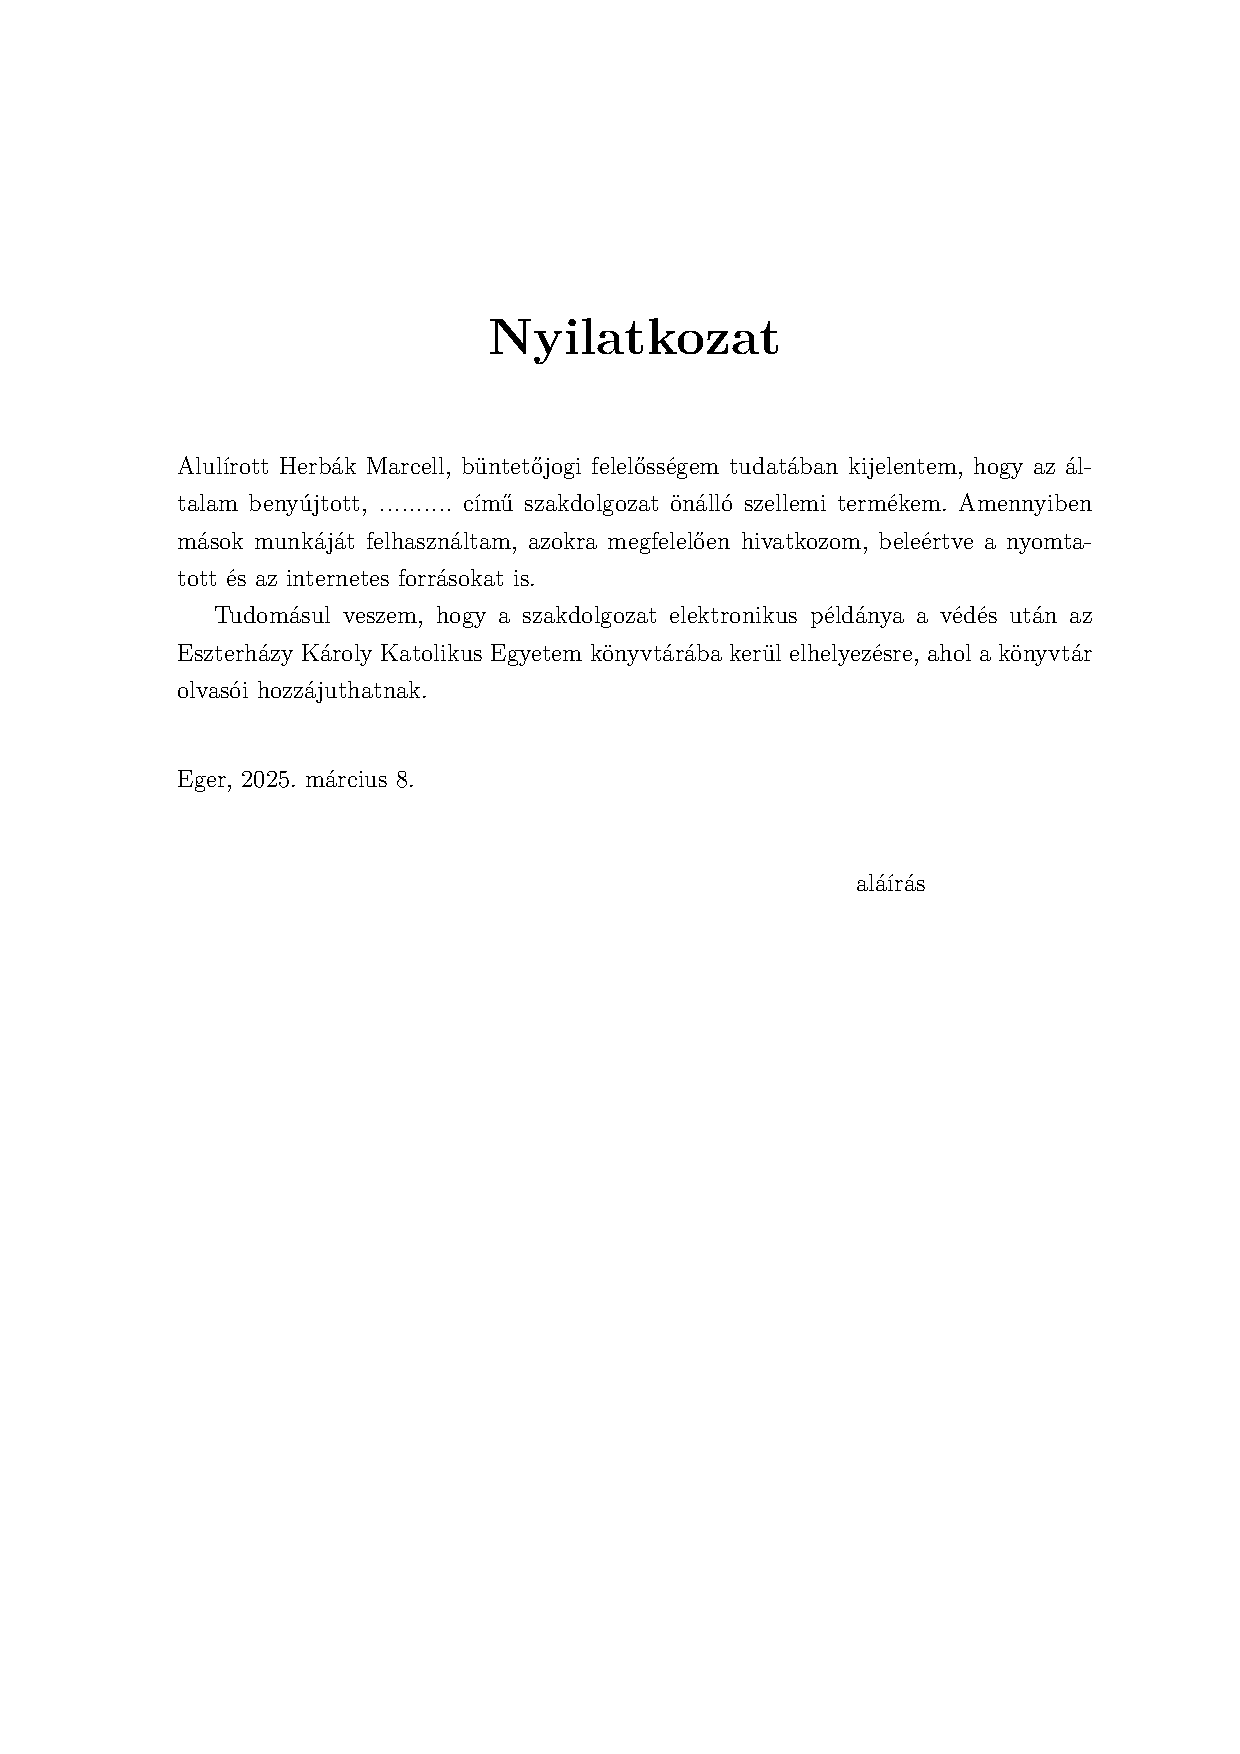
\includepdf{nyilatkozat/nyilatkozat.pdf}
\end{document}